\documentclass[twocolumn]{article}
\usepackage{calc}
\usepackage{ifthen}
\usepackage[margin=0.5in]{geometry}
\usepackage{amsmath,amsthm,amsfonts,amssymb}
\usepackage{amsfonts}
\usepackage{color,overpic}
\usepackage{hyperref}
\usepackage{array} 
\usepackage{amstext}
\usepackage{enumitem}
\usepackage{graphicx}
\usepackage{caption}
\usepackage{natbib}
\usepackage{framed}
\usepackage{enumitem}
\usepackage{float}
\usepackage{listings}


\newenvironment{Figure}
  {\par\medskip\noindent\minipage{\linewidth}}
  {\endminipage\par\medskip}
  
\numberwithin{equation}{section}


% Turn off header and footer
\pagestyle{empty}
\setlist[itemize]{leftmargin=*} % set itemise indentation to leftmargin
\setlist[enumerate]{leftmargin=*}

\title{Digital Signal Analysis}
\date{\vspace{-6ex}}

% -----------------------------------------------------------------------

\begin{document}
\maketitle


\newpage
\section{Tool}
	\subsection{Hilbert Space Interpretation}
Hilbert space is a generalisation of Euclidean space in higher dimension (even infinite dimension). It is define as a \textit{complete complex inner product} space. 
Square summable sequences is a special case of Hilbert space where $\|x\|=\sqrt{\sum_i \|x_i\|}$

	\subsection{Filter}
Filter is a process that removes from a signal some unwanted component. 

		\subsubsection{Time-domain}
A filter can be fully characterized by its impulse signal response. According to the response, filters can be categorise according to:
\begin{itemize}
	\item Finite Impulse Response (FIR) vs Infinite Impulse Response (IIR): finite (or infinite) duration.
	\item causal vs non-causal : causal use only past sample (impulse response is zero for n<0)
\end{itemize}

A bounded signal is whose value never exceed a finite value ($|y[n]|<B$). A BIBO (bounded-input, bounded-output) filter assure that a bounded input signal will produce a output bounded signal. The Fundamental Stalibity Theorem states that a filter is BIBO if and only if the impulse signal ($h[n]$) is absolutely integrable ($L^1$ norm exist)
$$ \sum_n|h[n]|=L<\infty \Leftrightarrow |y[n]|<B$$

		\subsubsection{Frequency-domain}
Magnitude classification of filter of pass-band frequency:
\begin{itemize}
	\item Low-pass : let only the low frequency pass ($<\omega_c$)
	\item High-pass : high freq.
	\item band-pass : compose of a low and high pass filter
	\item All-pass : constant magnitude 
	\item The Q-factor (quality) characterizes the bandwidth relative to its center ($f_c/\Delta f$).
\end{itemize}

\begin{figure}[H]
\centering
    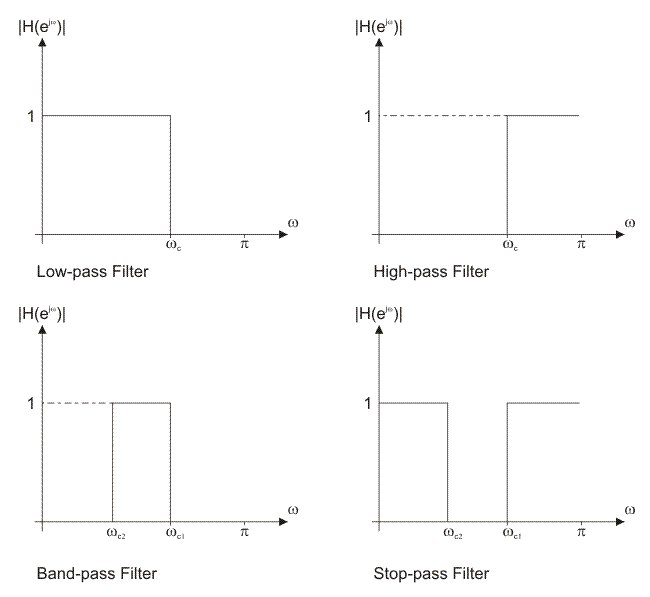
\includegraphics[width=.25\textwidth]{disco-house-types-of-filtering.png}
\end{figure}


		
	\subsection{Modulation}
Modulation is the process of varying properties of a periodic waveform ($x_c$, carrier signal) with a modulating signal ($x_m$) that contains information to be transmitted.
\begin{itemize}
	\item In Frequency modulation (FM), the carrier is sinusoidal $x_c(t) = A_c \cos (2 \pi f_c t)$ 
\end{itemize}



	\subsection{Perseval Theorem}
The theorem states that the inner product in time domain of two signal is equal to the inner product in frequency:
$$\langle f(x),g(x) \rangle = \langle \hat{f}(x),\hat{g}(x) \rangle $$
We can interpret this result as that the inner product is independent of the coordinate system. 

Taking the inner product of the signal itself, gives that the energy of a signal $E_{x} = \langle x(t), x(t)\rangle =  \int_{-\infty}^{\infty}{|x(t)|^2}dt$ remain the same when transform: 
$$\int_{-\infty}^\infty | x(t) |^2 \, dt   =   \int_{-\infty}^\infty | X(f) |^2 \, df  $$
	
	
	\subsection{Convolution} \label{subsec:convolution}
Convolution is an operation producing a modified function of the original one, giving the area overlap between the two functions as a function of the amount that one of the original functions is translated. Convolution is similar to cross-correlation but the signal is reversed. Autocorrelation is the convolution of the the signal itself.
$$ (f * g )(t) = \int_{-\infty}^\infty f(\tau) g(t - \tau) d\tau $$
Convolution is commutative ($f*g=g*f$), associative ($f*(g*h)=(f*g)*h$) and distributive ($f*(g+h)=(f*g)+(f*h)$).


The convolution theorem states that the Fourier transform of a convolution is the pointwise product of Fourier transforms. (convolution in time-domaine equal point-wise multiplication in frequency domain)
$$\mathcal{F}\{f*g\} = \mathcal{F}\{f\} \cdot \mathcal{F}\{g\}$$

	\subsection{Moving Average}
Moving average is a calculation to analyze data points by creating a series of averages of different subsets of the full data set.
$$y_M[n]=\frac{1}{M}\sum_{k=0}^{M-1} x[n-k]$$


	\subsection{L-p space}
The $L^p$-norm is defined :
$$\|\mathbf{x}\|_p := \bigg( \sum_{i=1}^n |x_i|^p \bigg)^{1/p}$$
The $L^p$-norm can be extended to vectors that have an infinite number of components, which yields the space $L^p$.

$L^p$ space may be defined as a space of function satisfaying:
$$\|f(x)\|_p \equiv \left({\int_S |f(x)|^p\;\mathrm{d} x}\right)^{\frac{1}{p}}<\infty$$
$L^ 1$, the space of sequences whose series is absolutely convergent,
$L^2$, the space of square-integrable function, which is a Hilbert space with inner product.


	\subsection{Shannon sampling theorem}
Sampling is the process of converting a signal into a numeric sequence.

Shannon sampling theorem establishes a sufficient sampling rate $\omega_s$ (in terms of the bandwidth) that permits to capture all the information in a signal when sampled. This signal need to have not Fourier transform frequencies above a certain value $B$ such that a sample rate spaced by $\omega_s \ge 2B$ can reconstruct all signal without any loss of information

When the bandlimit is too high (or there is no bandlimit), the reconstruction exhibits imperfections known as aliasing.
\begin{figure}[H]
\centering
    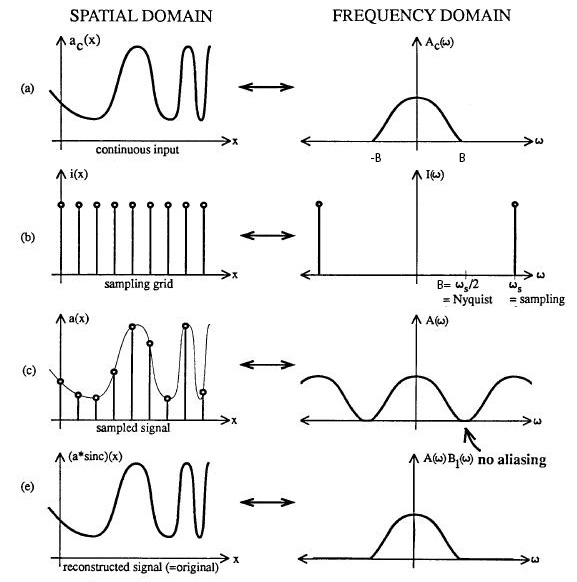
\includegraphics[width=.40\textwidth]{Sampl_Nyquist_F34.jpg}
\end{figure}


	\subsection{Complement and Supplement}
\begin{itemize}
	\item A complement of a set A refers to things not in A. 
	\item The relative complement of A with respect to a set B is the set of elements in B but not in A.
$$B \setminus A = \{ x\in B \, | \, x \notin A \}. $$
	\item The orthogonal complement $W^\bot$ of a subspace $W$ is the set of vector from $V$ which are orthogonal of all vector of $W$ 
$$W^\bot=\left\{\,x\in V\mid\forall y\in W\ \langle y \mid x \rangle = 0 \, \right\}.$$
	\item $F$ et $G$ are supplement (in $E$), denoted $F\oplus G = E$, if all vector in $E$ can be written uniquely as the sum of one vector of $F$ and one from $G$ :
$$\forall x\in E,\quad\exists ! (u,v)\in F\times G,\quad x=u+v.$$
\end{itemize}

	\subsection{Multiresolution analysis} \label{subsec:multiresolution_analysis}
A multiresolution analysis of $L^2(\mathbb R )$ consists of a sequence $\{V_j\}_{j\in \mathbb Z}$ of closed nested subspaces such that:
\begin{enumerate}[label=(\roman*)]
	\item $\{V_j\}_{j\in \mathbb Z}$ is a closed subspace of $L^2(\mathbb R )$
	\item Nested: $V_{j-1}\subset V_j$
	\item $V_j$ fill up all $L^2(\mathbb R )$: $\overline{\bigcup\limits_{j\in \mathbb Z} V_{j}}=L^2(\mathbb R )$ and are not redundant: $\bigcap\limits_{j\in \mathbb Z} V_{j}=\{0\}$
	\item Each subspace $V_j$ is invariant under shifts by integer multiples of $2^j$: $f(x)\in V_j \Rightarrow f(x-m2^{j}) \in V_j$
	\item All subspaces $V_j\subset V_l,\; j>l$, are time-scaled versions of each other:  $f(x)\in V_j  \Rightarrow f(2^{j-l}x) \in V_l$
\end{enumerate}

	\subsection{Refinable function} \label{subsec:refinable-function}
A function $\varphi$ is called refinable with respect to the mask $h$ if
$$\varphi(x)=2 \sum_{k=0}^{N-1} h_k \varphi(2 x-k)=2 D_{1/2} (h * \varphi)$$
Where $D$ is the dilation operator and $*$ the convolution (see subsection~\ref{subsec:convolution}). This condition is called two-scale equation.
	
	\subsection{Filter Bank Theory}
	
	

\newpage
\section{Fourier Transform}
Its definition is quite simple : "Fourier analysis is the study of the way general functions may be approximated by sums of simpler trigonometric functions"
	
	\subsection{Continuous} 
\begin{framed}
Be an integrable function $f : \mathbb R \rightarrow \mathbb C$, its Fourier transform $\hat{f}$ and back transform $f$ are defined:

\begin{align*}
\hat{f}(\xi) &= \int_{-\infty}^\infty f(x)\ e^{- 2\pi i x \xi}\,dx= 
\frac{1}{\sqrt{2 \pi}} \int_{-\infty}^{\infty} f(x) e^{-i \omega x}\, dx \\
f(x) &= \int_{-\infty}^\infty \hat f(\xi)\ e^{2 \pi i \xi x}\,d\xi, = \frac{1}{\sqrt{(2 \pi)}} \int \hat{f}
(\omega)e^{i \omega\cdot x}\, d\omega
\end{align*}
When $x$ represent time, $\xi$ represent frequency and $\omega$ the 
\end{framed}

Fourrier transform is linear, bijective, continue and conserve angle and length. 
Properties
\begin{enumerate}
\item Linearity: $h(x)=a\cdot f(x) + b\cdot g(x) \Rightarrow \hat{h}(\xi)=a\cdot \hat{f}(\xi) + b\cdot\hat{g}(\xi)$
\item Time shift: $h(x)=f(x-x_0) \Rightarrow \hat{h}(\xi)= e^{-i\,2\pi \,x_0\,\xi }\hat{f}(\xi)$
\item Modulation:  $h(x)=e^{i \, 2\pi \, x \,\xi_0}f(x)\Rightarrow  \hat{h}(\xi) = \hat{f}(\xi-\xi_{0})$
\item Time conjugation $h(x)=\overline{f(x)}\Rightarrow  \hat{h}(\xi) = \overline{\hat{f}(-\xi)}.$
\end{enumerate}



	\subsection{Fourier Series}
$s(x)$ denotes a function integrable on $[x_0,x_0+P]$ which can be approximate with $s_N(x)$ a series N sinus.
\begin{align*}
s_N(x) 	&= \frac{A_0}{2} + \sum_{n=1}^N A_n\cdot \sin(\tfrac{2\pi nx}{P}+\phi_n) \\
		&\approx \frac{a_0}{2} + \sum_{n=1}^N \left(\overbrace{a_n}^{A_n \sin(\phi_n)} \cos(\tfrac{2\pi nx}{P}) + \overbrace{b_n}^{A_n \cos(\phi_n)} \sin(\tfrac{2\pi nx}{P})\right)\\
		&\approx \sum_{n=-N}^N c_n\cdot e^{i \tfrac{2\pi nx}{P}},
\end{align*}
$a_n$, $b_n$ and $c_n$ are known as the Fourier coefficient and defined:
\begin{align*}
a_n &= \frac{2}{P}\int_{x_0}^{x_0+P} s(x)\cdot  \cos(\tfrac{2\pi nx}{P})\ dx\\
b_n &= \frac{2}{P}\int_{x_0}^{x_0+P} s(x)\cdot  \sin(\tfrac{2\pi nx}{P})\ dx\\
c_n &= \frac{1}{P}\int_{x_0}^{x_0+P} s(x)\cdot e^{-i \tfrac{2\pi nx}{P}}\ dx\\
\end{align*}

	\subsection{Discrete Fourier Transform (DFT)}
\begin{framed}
The sequence $x_n \in \mathbb{C}$ with $n=\{0,N-1\}$ is transformed into a other sequence $X_k \in \mathbb{C}$ with $k=\{0,N-1\}$ :
$$ X_k = \sum_{n=0}^{N-1} x_n  e^{-i \frac{2 \pi k}{N} n},  \quad k\in \{0, N-1\}$$
$$ x_n = \frac{1}{N} \sum_{k=0}^{N-1} X_k e^{-i \frac{2 \pi }{N} nk},  \quad n\in \{0, N-1\}$$
\end{framed}
This can be view:
\begin{enumerate}
	\item A Hilbert space basis transformation: projection of $x$ on the vector space $w_n^k = e^{ i \frac{2\pi }{N} kn}$ such that: $ X_k = \langle w_n^k , x_n \rangle$
	\item Matrix Notation : $  \boldsymbol{X} = \boldsymbol{W} \boldsymbol{x}$
	\item The discrete analogy of the formula for the coefficients of a Fourier series:
	\item The cross-corelation of a input sequence $x_n$ and a complex sinusoid at frequency $k/N$ (a sort of matching filter). 
\end{enumerate} 

Properties
\begin{enumerate}
	\item Completeness: DFT is an invertible. $\mathcal{F}\colon\mathbb{C}^N \to \mathbb{C}^N$
	\item Orthogonality: $\langle \boldsymbol{w}^{(k)} , \boldsymbol{w}^{(h)} \rangle =\sum_{n=0}^{N-1} e^{j\frac{2 \pi}{N}n(h-k)}=\frac{1-e^{j2 \pi (h-k)}}{1-e^{j \frac{2 \pi}{N} (h-k)}}=0$
	\item with Perseval theorem, concervation of energy ???
	\item Periodicity: $X_{k+N} = \sum_{n=0}^{N-1} x_n e^{-\frac{2\pi i}{N} (k+N) n} = X_k. $
\end{enumerate} 



	\subsection{Discrete Fourier Serie (DFS)}
Discrete Fourier Serie (DFS) is the equivalent to the DFT for a period input signal. The equation are the same except that $k \in \mathbb{Z}$ for the forward and $n \in \mathbb{Z}$ for the backward. The tilde notation is used for it $\tilde{x}$, $\tilde{X}$.

%DFS is helpful for time shift:
%$$DFS\{\tilde{x}_{n-M}\}=e^{-i\frac{2\pi}{N}Mk\tilde{X}_k$$


	\subsection{Discrete-Time Fourier Transform (DTFT)}
\begin{framed}
The Discrete-Time Fourier Transform (DTFT) of a discrete set  $x[n] \in \mathbb{C}$ with $n \in \mathbb{Z}$ and square summable $x[n] \in l_2(\mathbb{Z})$ is a Fourier series which produces a periodic function $ F(\omega), \quad \omega \in \{0,2\pi\}$.

$$X(e^{i\omega}) = \langle e^{i\omega n},x[n] \rangle = \sum_{n=-\infty}^{\infty} x[n] \,e^{-i \omega n}$$

 $$x[n] = \frac{1}{2\pi}\int_{-\pi}^{\pi} X(e^{i\omega}) \,e^{i \omega n} d\omega$$
\end{framed}


For a N-singal $x[n]$, $X[k]$ is found with DFT but how to extend it to infinity and use the DTFT ?
$$\tilde{x}=x[n \text{mod} N] \quad \rightarrow \quad \tilde{X}(e^{i\omega})=\frac{1}{N} \sum_{k=0}^{N-1} X[k] \tilde{\delta}(\omega - \frac{2 \pi}{N}k)$$
$$\bar{x}=x[n] n<N  \quad \rightarrow \quad \tilde{X}(e^{i\omega})=\frac{1}{N} \sum_{k=0}^{N-1} X[k] \tilde{\delta}(\omega - \frac{2 \pi}{N}k)$$


	\subsection{Fast Fourier Transform (FFT)}


	\subsection{2D image}
$$X[k_1,k_2]= \sum_{n_1=0}^{N_1 -1} \sum_{n_2=0}^{N_2 -1} x[n_1,n_2] e^{-j \frac{2 \pi}{N_1}n_1 k_1}  e^{-j \frac{2 \pi}{N_2}n_2 k_2}$$
$$x[n_1,n_2]= \frac{1}{N_1 N_2} \sum_{k_1=0}^{N_1 -1} \sum_{k_2=0}^{N_2 -1} X[k_1,k_2] e^{j \frac{2 \pi}{N_1}n_1 k_1}  e^{j \frac{2 \pi}{N_2}n_2 k_2}$$
They are $N_1 \times N_2$ basis vectors:
$$w_{k_1,k_2}[n_1,n_2]=e^{j \frac{2 \pi}{N_1}n_1 k_1}  e^{j \frac{2 \pi}{N_2}n_2 k_2}$$



	\subsection{Inconvenient of Fourier Analysis}
\begin{enumerate}
	\item Lost of temporal aspect
	\item Impossibility to do on-time transform, need the full data.
	\item Uncertainty principal of Heisenberg: impossible to assign simultaneously an exact time and frequency response.
\end{enumerate}


	\subsection{Short-Time Fourier Transform (STFT)}
If we desire to keep information of both time of occurrence and frequency, the STFT is splitting the signal in m small pieces of length L
$$X[m,k]=\sum_{n=0}^{L-1} x[m+n]e^{-j\frac{2 \pi}{L}nk}$$
This method is used to plot the spectrogram (frequency vs time vs amplitude). The windows determines whether there is good frequency resolution (wide window, more point, frequency components close together can be separated) or good time resolution (narrow windows, the time at which frequencies change). These are called narrowband and wideband transforms, respectively.

In continuous-time, we use a windows function which restreint the analysis around a certain point $\tau$

$$ X(\tau, \omega) = \int_{-\infty}^{\infty} x(t) w(t-\tau) e^{-j \omega t} \, dt $$

	\subsection{Gabor transform}
The Gabor transform has a windows function $w=e^{-\pi(t-\tau)^2}$ which is equal to its own Fourier transform.
$$ G_x(\tau,\omega) = \int_{-\infty}^\infty x(t)e^{-\pi(t-\tau)^2}e^{-j\omega t}\,dt $$

\begin{figure}[H]
\centering
    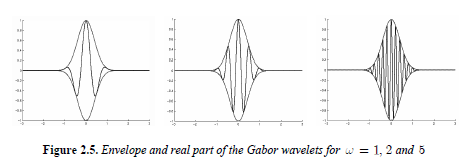
\includegraphics[width=.49\textwidth]{img26.png}
\end{figure}

$\omega$ controle the number of oscillation and $\tau$ the temporal location, but the envelope remain the same.


\newpage
	\section{Wavelet Transform}
		\subsection{Introduction}
			\subsubsection{History}
\begin{itemize}
	\item Haar (1910) \ref{} constructed the the first wavelet (Haar wavelet),
$$\psi(t) = \begin{cases}
  1 \quad & 0 \leq  t < \frac{1}{2},\\
 -1 & \frac{1}{2} \leq t < 1,\\
  0 &\mbox{otherwise.}
\end{cases}$$
	\item In 1980, Stromberg create a second wavelet \ref{}
	\item Mayer in an attempt to demonstrate that there is no regular wavelet which generate an orthogonal basis, end up constructed a whole family of wavelet \ref{} later called Daubechies.
	\item Mayer and Mallat established the systematic theory of wavelet construction with multiresolution signal approximation 
	\item Fast Wavelet Transform Algorithm O(N) opperation.
\end{itemize}

3 applications: Analysis of a signal, noise removal and compression. 
			\subsubsection{Reasoning}
The Short-Time Fourier Transform are useful but the windows (or envelope) remain the same. Multi-resolution analysis (MRA) help us to analyse a signal at different frequencies with different resolutions. As it is often the case in signal, high frequency components have short durations and low frequency components have longer durations, it makes sense to have good time resolution and poor frequency resolution at high frequencies and good frequency resolution and poor time resolution at low frequencies.
\begin{figure}[H]
\centering
    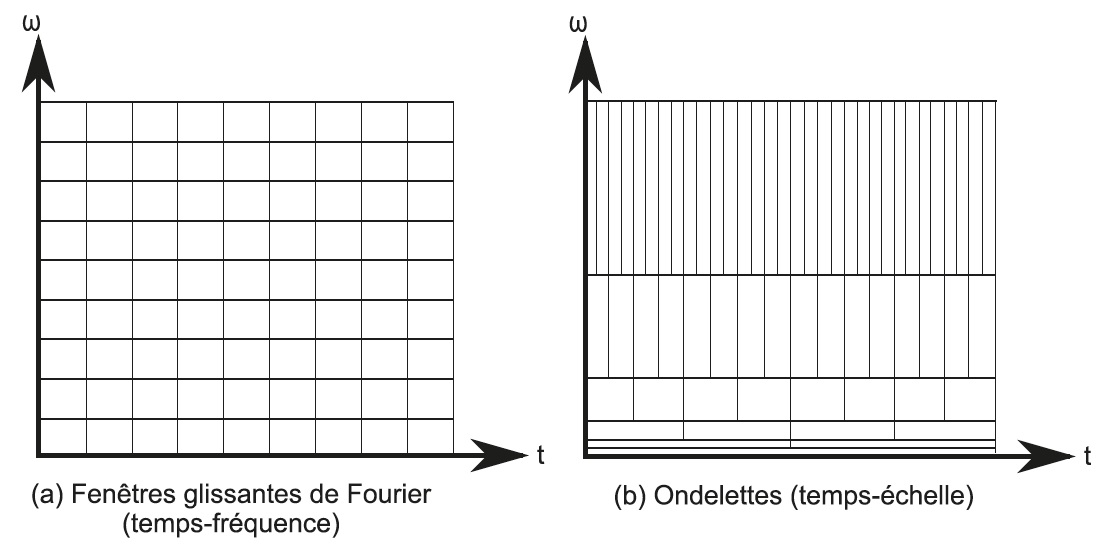
\includegraphics[width=.40\textwidth]{500px-STFT_and_WT.jpg}
\end{figure}
		\subsection{Mother Wavelet}
A mother wavelet is a function $\psi (t)$ from measurable and square integrable functions space  $L^1\cap L^2$ and must verify the \textit{admissibility condition}:
$$ \int\frac{|\hat{\psi}(\omega)|^2}{|\omega|}d\omega < \infty$$
This minimial condition need to be reinforce by admitting n+1 moments nuls (vanishing moments). This force the signal to be fast decaying:
$$\int_{-\infty}^{\infty} t^p\,\psi (t)\, dt = 0 \quad \text{for }p=0,...n$$
or event more simpler (and often used):
$$ \psi \in \mathbb{R}, \quad \psi \in L^1\cap L^2, \quad t \psi  \in L^1, \quad  \int_{\mathbb{R}} \psi (t) dt=0$$

		\subsection{Children wavelet}
This mother wavelet is scaled (or dilated) by a factor of $s$ and translated (or shifted) by $\tau$ to give child wavelet or atom:

$$\boxed{\psi _{\tau,s} (t) = {1 \over \sqrt s}\psi \left( {t -\tau \over s} \right)}$$

$|s|^{-1/2}$ is the energy normalization. This transformation preserve energy ($\|\psi\|_2=\|\psi _{\tau,s}\|_2$)
\begin{figure}[H]
\centering
    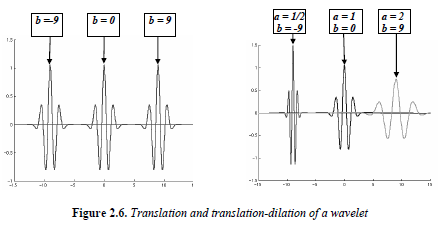
\includegraphics[width=.40\textwidth]{img27.png}
    \includegraphics[width=.20\textwidth]{mallat2.png}
\end{figure}

		\subsection{Continuous wavelet transforms (CWT)}
CWT of $f(t)$ is composed of the coefficient $CWT_f^\psi(\tau,s)$ created by convolution of $f$ with the different children wavelet:
$$\boxed{CWT_f^\psi(\tau,s)=\langle f,\,\psi_{\tau,s}\rangle=\frac{1}{|s|^{1/2}} \int_{-\infty}^{\infty} f(t)\overline\psi\left(\frac{t-\tau}{s}\right)\, dt}$$

And its inverse is:
$$f(t)=C_\psi^{-1}\int_{-\infty}^{\infty}\int_{-\infty}^{\infty} C_f(\tau,s)\psi _{\tau,s} d\tau \frac{ds}{s^2}$$
with $C_\psi = \int_{-\infty}^{+\infty}
  \frac{\left| \hat{\psi}(\omega) \right|^2}{\left| \omega \right|} d\omega$
  
		\subsection{Discrete wavelet transforms (DWT)}
DWT recognized the redundancy and infinite number of wavelet in the CWT. With DWT, we are choosing finite discrete $s=s_0^j$ and $\tau=k\tau_0 s_0^j$:
$$\psi_{j,k}(t)=\frac{1}{\sqrt{s_0^{j}}} \psi\left(\frac{t-k\tau_0 s_0^j}{s_0^j}\right)$$
Because of the Shannon sampling theorem (dyadic sampling) it is very common to take $s_0=2$ and $\tau_0=1$
$$\psi_{j,k}(t)=\frac{1}{\sqrt{2^{j}}} \psi\left(\frac{t-k 2^j}{2^j}\right)$$

The DWT coefficient are calculated with:

$$\boxed{DWT_f^{\psi}(j,k)=\langle f,\,\psi_{j,k}\rangle=\frac{1}{\sqrt{2^{j}}}  \int_{-\infty}^{\infty} f(t)\overline\psi\left(\frac{t-k 2^j}{2^j}\right)\, dt}$$



		\subsection{Reconstruction}
A sufficient condition for the reconstruction is that energy of the wavelet coefficient must be bounded:
$$ A\|f\|^2 \le \sum |\langle f,\,\psi_{\tau,s}\rangle|^2 \le B\|f\|^2$$
In this case $\psi_{\tau,s}$ can be refer as a frame (basis function which can be dependent). When the frame is tight $A=B$, the wavelet behave as an orthonormal basis. Reconstruction of the function is done with
$$ f=\sum_{j,k}\langle f,\,\psi_{\tau,s}\rangle\cdot\psi_{\tau,s}$$.

When the frame is not tight, reconstruction is still possible but at the cost of a dual frame. In this case, the decomposition wavelet is different from the reconstruction wavelet. None-orthogonal wavelet can be useful in their redundancy. 

However, it is common to choose a orthonormal mother wavelet:
$$\langle \psi_{m,n},\,\psi_{j,k}\rangle = \left\{
  \begin{array}{ll}
    1 & \text{if } j=m \text{ and } k=n\\
    0 & \text{otherwise}
  \end{array}
\right. $$
Note that, in this case, only DWT can be used.

		\subsection{Filtering approch}
If a wavelet can be viewed as a band-pass filter (with a constant Q-factor), covering the whole signal require an infinite number of wavelet (as the wavelet stretch in time domain, his bandwidth stretch and more wavelet are required)

The solution is to use a low-pass filter called scaling function $\varphi_{j,k}(t)$ which cover all lower frequency such that
$$\varphi_{J,k}(t)=\sum_{j, j>J} \psi_j(t)$$
\begin{figure}[H]
\centering
    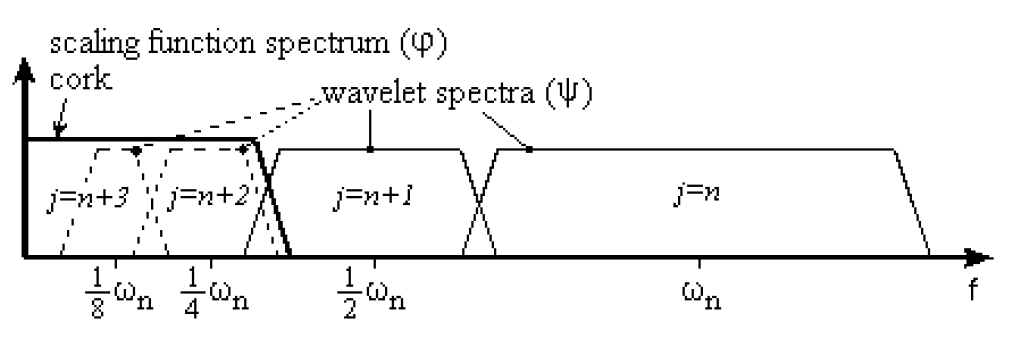
\includegraphics[width=.49\textwidth]{wavelet_scaling_function.png}
\end{figure}

		\subsection{Multiresolution analysis}
			\subsubsection{Approximation and detail space}
We define a two multiresolution (see subsection~\ref{subsec:multiresolution_analysis}) sequences of subspace $\{V_j\}_{j\in \mathbb Z}$ and $\{W_j\}_{j\in \mathbb Z}$, where $W_j$ (\textit{detail} space) is the orthogonal supplement of $V_j$(\textit{approximation} space) in $V_{j-1}$ denoted 
$$V_{j-1}=V_j \oplus W_j \quad \text{with } W_j \perp V_j$$
This relation imply different consequences
\begin{enumerate}[label=(\roman*)]
	\item A subspace $V_j$ can be express as a combination of space
	$$V_J=V_K \oplus W_K \oplus \cdots \oplus W_{J-1}=\bigoplus_{j=J+1}^\infty W_j, \quad \text{with } J < K$$
	\item The full space $L^2(\mathbb R )$ is therefore decompasable in:
	$$L^2(\mathbb R )=V_J \oplus \left \{ \bigoplus_{j=-\infty}^J W_j\right \}=\bigoplus_{j=-\infty}^\infty W_j$$ 
\end{enumerate}



		\subsection{Orthogonal Basis}

Using the detail and approximation space space, let $\left\{ \psi_{j,k} \right\}_{k\in \mathbb{Z}}$ be an orthogonal basis generating $W_j$ while $\left\{ \varphi_{j,k} \right\}_{k\in \mathbb{Z}}$ generate $V_j$.  

As $L^2(\mathbb R )=\bigoplus_{j=-\infty}^\infty W_j$,  $\left\{ \psi_{j,k} \right\}_{j,k\in \mathbb{Z}}$ can generate all $L^2(\mathbb R)$ and any signal $f(t)$ can be decompose and reconstruct using this wavelet basis. 

Together, $\forall J \in \mathbb{Z}, \left\{ \left\{ \varphi_{J,k} \right\}_{k\in \mathbb{Z}}, \left\{ \psi_{j,k} \right\}_{j,k\in \mathbb{Z},j\le J} \right\}$ is an orthonormal basis of $L^2(\mathbb R )$
\begin{figure}[H]
\centering
    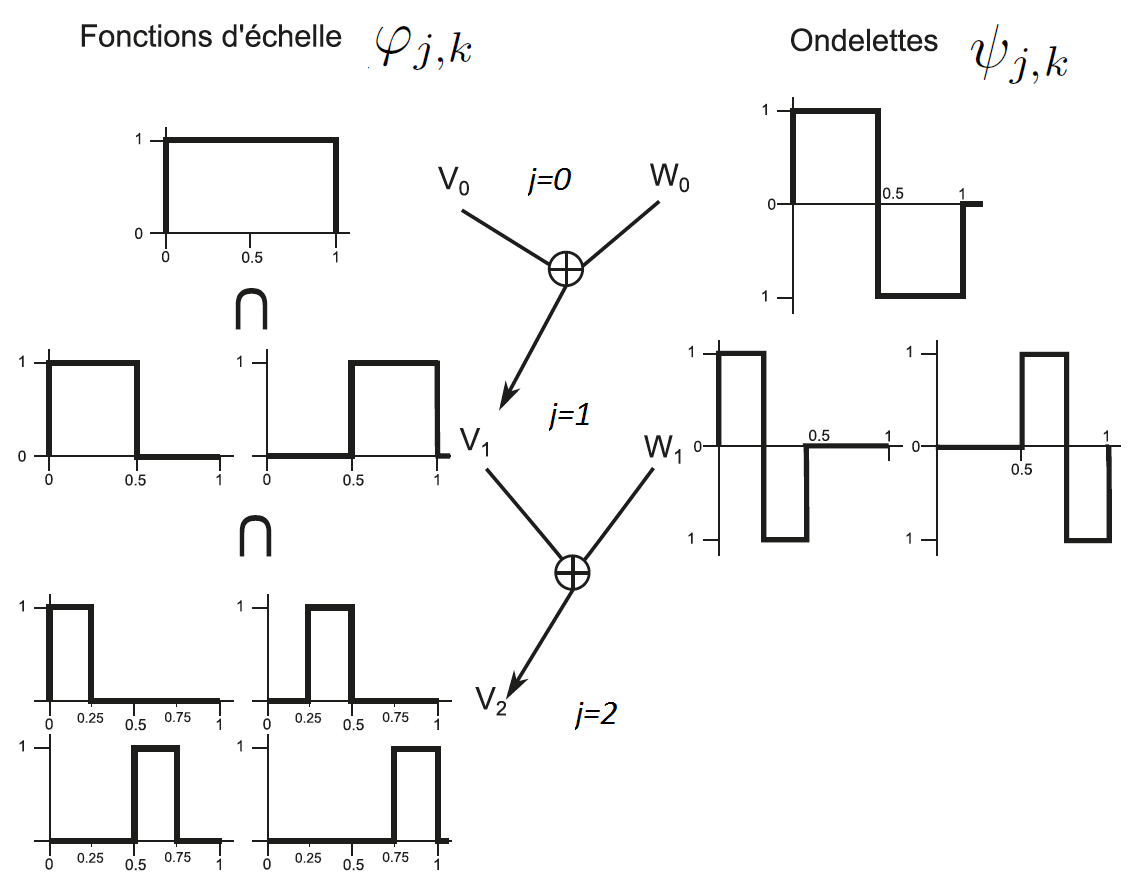
\includegraphics[width=.49\textwidth]{WVjk.png}
\end{figure}

		\subsection{Two-scale relation}
We know intuitively that a scaling function at scale $j$ is a linear combinaison of the scaling function at scale $j+1$. This can be formulated with the two-scale relationship and the scalling fonction is called refinable (see subsection~\ref{subsec:refinable-function}):
$$\varphi_{j,k}=2\sum_{k\in \mathbb{Z}}h_{j,k} \varphi_{j+1,k} \quad \text{or}\quad \frac{1}{2}\varphi\left(\frac{t}{2}\right)=\sum_{k\in \mathbb{Z}}h_k \varphi(t-k)$$

Because the scaling function at scale $j$ ....
$$\psi_{j,k}=2\sum_{k\in \mathbb{Z}}g_{j,k} \varphi_{j+1,k}$$
		\subsection{Construction and }
		
For all function $f$ in $L^2(\mathbb R)$, the projection on $V_j$ and $W_j$ are denoted $A^j=P_{V_j}f$ and $D^j=P_{W_j}f$.

$$A^{J-1}=A^J +D^J \quad \text{and} \quad f=A^J + \sum_{-\infty}^J D^j$$
We can interpreted this as that all detail $D^j$ need to be added to the approximation $A^J$ to reconstruct the function $f$

The computation of this projection is done by first computing coefficient:
$$\alpha_{j,k}=\int_\mathbb{R} f(t) \psi_{j,k}(t) \quad \text{and} \quad \beta_{j,k}=\int_\mathbb{R} f(t) \varphi_{j,k}(t)$$
$$D_j(t)=\sum_{k \in \mathbb{Z}} \alpha_{j,k} \psi_{j,k}(t) \quad \text{and} \quad A_j(t)=\sum_{k \in \mathbb{Z}} \beta_{j,k} \varphi_{j,k}(t)$$
The more formal approach to express discrete filter wavelet transform is by using multi-resolution analysis.




Because of property (v) of the approximation space, 
$$\varphi_{j,k}(t)=2^{j/2}\varphi(2^j t-k) $$
$$\varphi_{j,k}(t) =\sum_l h_{\varphi}[l] \varphi_{j+1,l}(t)=\sum_l h_{\varphi}[l] 2^{(j+1)/2} \varphi(2^{j+1}t-l)$$

$$f(t)=\sum_k c_{j_0,k}\varphi_{J,k}(t)+\sum_{j=J}^{\infty} \sum_k d_{j,k}\psi_{j,k}(t)$$



		\subsection{Wavelet for Images}
\bibliographystyle{apalike}
\bibliography{citations}
	

\end{document}
